\documentclass[table]{beamer}

\title{Using the internal language of toposes in algebraic geometry}
\author{Ingo Blechschmidt}
\institute{University of Augsburg}
\date{June 23th, 2014}

\usepackage[english]{babel}
\usepackage[protrusion=true,expansion=true]{microtype}
\usepackage{amsmath,amsfonts,amssymb,amsthm}
\usepackage{tikz}
\usepackage{booktabs}
\usepackage{ragged2e}
\usepackage[orientation=landscape,size=a2,scale=0.8]{beamerposter}

\usefonttheme{professionalfonts}
\usepackage{pxfonts}

\definecolor{lgreen} {RGB}{180,210,100}
\definecolor{dblue}  {RGB}{20,66,129}
\definecolor{ddblue} {RGB}{11,36,69}
\definecolor{lred}   {RGB}{220,0,0}
\definecolor{nred}   {RGB}{224,0,0}
\definecolor{norange}{RGB}{230,120,20}
\definecolor{nyellow}{RGB}{255,221,0}
\definecolor{ngreen} {RGB}{98,158,31}
\definecolor{dgreen} {RGB}{78,138,21}
\definecolor{nblue}  {RGB}{28,130,185}
\definecolor{jblue}  {RGB}{20,50,100}

\setbeamercolor{palette primary}   {fg=black,bg=white}
\setbeamercolor{palette secondary} {fg=black,bg=white}
\setbeamercolor{palette tertiary}  {bg=jblue,fg=white}
\setbeamercolor{palette quaternary}{fg=black,bg=white}
\setbeamercolor{structure}{fg=jblue}
\setbeamercolor{titlelike}         {bg=jblue,fg=white}
\setbeamercolor{frametitle}        {bg=jblue!10,fg=jblue}
\setbeamercolor{cboxb}{fg=black,bg=jblue}
\setbeamercolor{cboxr}{fg=black,bg=red}

\setbeamercolor{item}{fg=ngreen}
\setbeamercolor{item projected}{fg=white,bg=ngreen}

\setbeamercolor{block title}{fg=nred,bg=white}
\setbeamercolor{block body}{fg=black,bg=white}

\setbeamercolor{block alerted title}{fg=white,bg=jblue}
\setbeamercolor{block alerted body}{fg=black,bg=jblue!10}

\setbeamerfont{section in head/foot}{series=\bfseries}
\setbeamerfont{block title}{series=\bfseries}
\setbeamerfont{block alerted title}{series=\bfseries}
\setbeamerfont{frametitle}{series=\bfseries}
\setbeamerfont{frametitle}{size=\Large}
\setbeamerfont{block body}{series=\rmfamily}

\setbeamertemplate{items}[circle]
\setbeamertemplate{blocks}[width=0.0]
\beamertemplatenavigationsymbolsempty

\makeatletter
\newenvironment{beamercolorboxA}[2][]{%
  \begingroup%
    \def\beamer@colbox@coladd{0pt}%
    \def\beamer@vmode{\leavevmode}%
    \setkeys{beamercolbox}{%
      wd=\textwidth,ht={},dp={},%
      leftskip=0pt,rightskip=0pt plus1fil,%
      sep=0pt,colsep=0pt,colsep*=0pt,%
      shadow=false,rounded=false,ignorebg=false}%
    \setkeys{beamercolbox}{#1}%
    \ifbeamercolorempty[bg]{#2}{\@tempswafalse}{\@tempswatrue}%
    \ifbeamer@colbox@ignorebg\@tempswafalse\fi%
    \def\beamer@colbox@color{#2}%
    \hsize=\beamer@colbox@wd%
    \setbox\beamer@tempbox=\hbox\bgroup\vbox\bgroup%
      \leftskip=\beamer@colbox@ls%
      \advance\leftskip by\beamer@colbox@sep%
      \rightskip=\beamer@colbox@rs%
      \advance\rightskip by\beamer@colbox@sep%
      \ifbeamer@colbox@ignorebg%
        \colorlet{beamer@temp@color}{bg}%
        \usebeamercolor[fg]{#2}%
        \colorlet{bg}{beamer@temp@color}%
      \else%
        \usebeamercolor[fg]{#2}%
      \fi%
      \if@tempswa%
        \advance\leftskip by\beamer@colbox@colsep%
        \advance\rightskip by\beamer@colbox@colsep%
        \ifdim\beamer@colbox@colsep=0pt\else\vskip\beamer@colbox@colsep\fi%
        \ifdim\beamer@colbox@colseps=0pt\else\vskip\beamer@colbox@colseps\fi%
      \fi%
      \ifdim\beamer@colbox@sep=0pt\else\vskip-0.3cm\fi%
      \beamer@vmode\ignorespaces}{%
      \ifdim\beamer@colbox@sep=0pt\else\vskip\beamer@colbox@sep\fi%
      \if@tempswa\ifdim\beamer@colbox@colsep=0pt\else\vskip\beamer@colbox@colsep\fi\fi%
      \if@tempswa\ifdim\beamer@colbox@colseps=0pt\else\vskip\beamer@colbox@colseps\fi\fi%
    \egroup\egroup%
    \wd\beamer@tempbox=\hsize%
    \@tempdima=\wd\beamer@tempbox%
    \ifx\beamer@colbox@ht\@empty%
    \else%
      \ht\beamer@tempbox=\beamer@colbox@ht%
    \fi%
    \ifx\beamer@colbox@dp\@empty%
    \else%
      \dp\beamer@tempbox=\beamer@colbox@dp%
    \fi%
    \ifbeamer@colbox@rounded%
      \if@tempswa%
        \begin{beamerboxesrounded}[%
          shadow=\beamer@colbox@shadow,%
          lower=\beamer@colbox@color,%
          upper=normal text,%
          width=\beamer@colbox@wd]{}%
          \box\beamer@tempbox%
        \end{beamerboxesrounded}%
      \else%
        \ifdim\@tempdima>\textwidth%
          \setbox\beamer@tempbox=\hbox to\textwidth{\hss\box\beamer@tempbox\hss}%
        \fi%
        \box\beamer@tempbox%
      \fi%
    \else%
      \if@tempswa\setbox\beamer@tempbox=\hbox{\vbox{%
        \usebeamercolor{\beamer@colbox@color}%
        \advance\hsize by \beamer@colbox@colseps\relax%
        \advance\hsize by \beamer@colbox@colseps\relax%
        \hskip-\beamer@colbox@colseps%
        \fboxsep=0pt\colorbox{bg}{%
          \hskip\beamer@colbox@colseps%
          \hbox{\box\beamer@tempbox}%
          \hskip\beamer@colbox@colseps%
        }%
        \hskip-\beamer@colbox@colseps%
      }}\fi%
      \ifdim\@tempdima>\textwidth%
        \setbox\beamer@tempbox=\hbox to\textwidth{\hskip0pt minus\beamer@leftmargin\relax\box\beamer@tempbox\hskip0pt minus\beamer@rightmargin\relax}%
      \fi%
      \box\beamer@tempbox%
    \fi%
  \endgroup%
}
\makeatother

\setbeamertemplate{block begin}
{
  \par\vskip\medskipamount
  \begin{beamercolorbox}[colsep*=0ex,dp={2ex},center]{block title}
    \vskip-0.25cm
    \usebeamerfont{block title}\large\insertblocktitle
    \begin{flushleft}
    \vskip-0.8em
    \begin{tikzpicture}[remember picture,overlay]
      \shade [inner color=gray,outer color=white]
      (0,0) rectangle (\textwidth,0.3cm);
    \end{tikzpicture}
    \end{flushleft}
  \end{beamercolorbox}
  {\parskip0pt\par}
  \ifbeamercolorempty[bg]{block title}
  {}
  {\ifbeamercolorempty[bg]{block body}{}{\nointerlineskip\vskip-0.5pt}}
  \usebeamerfont{block body}
  \vskip-0.5cm
  \begin{beamercolorbox}[colsep*=0ex,vmode]{block body}
  \justifying
}

\setbeamertemplate{block end}
{
  \end{beamercolorbox}
  \vskip\smallskipamount
}

\newlength{\inboxwd}
\newlength{\iinboxwd}
\setbeamertemplate{block alerted begin}
{
  \par\vskip\medskipamount
  \begin{beamercolorbox}[sep=0ex,rounded=true,center,dp={2.0ex}]{block alerted title}
    \vskip-0.2cm
    \usebeamerfont{block title}\large\insertblocktitle
    \vskip0.05cm
  \end{beamercolorbox}
  {\parskip0pt\par}
  \usebeamerfont{block body}
  \vskip-0.5cm
  \begin{beamercolorboxA}[sep=0.5cm, rounded=true,center]{block alerted title}
  \setlength{\inboxwd}{\linewidth}
  \addtolength{\inboxwd}{-1cm}
  \begin{beamercolorbox}[rounded=true,wd={\inboxwd},center]{block alerted body}
  \setlength{\iinboxwd}{\inboxwd}
  \addtolength{\iinboxwd}{-0.5cm}
  \begin{center}
  \begin{minipage}{\iinboxwd}
  \justifying
}

\setbeamertemplate{block alerted end}
{
  \end{minipage}
  \end{center}
  \end{beamercolorbox}
  \end{beamercolorboxA}
  \vskip\smallskipamount
}

\setbeamertemplate{headline}{
 \leavevmode
  \begin{columns}
   \begin{column}{\linewidth}
    \vskip1cm
    \centering
    \usebeamercolor{title in headline}{\color{jblue}\huge{\textbf{\inserttitle}}\\[0.5ex]}
    \usebeamercolor{author in headline}{\color{fg}\large{\insertauthor},}
    \usebeamercolor{institute in headline}{\color{fg}\large{\insertinstitute}\\[1ex]}
    \vskip1cm
   \end{column}
   \vspace{1cm}
  \end{columns}
 %\hspace{0.5in}\begin{beamercolorbox}[wd=\linewidth,colsep=0.15cm]{cboxb}\end{beamercolorbox}
 %\vspace{0.1in}
}

\newcommand{\E}{\mathcal{E}}
\newcommand{\F}{\mathcal{F}}
\newcommand{\G}{\mathcal{G}}
\renewcommand{\H}{\mathcal{H}}
\renewcommand{\O}{\mathcal{O}}
\newcommand{\K}{\mathcal{K}}
\newcommand{\Sh}{\mathrm{Sh}}

\begin{document}

\begin{frame}[t]\begin{columns}[t]

\begin{column}{0.3\textwidth}
  \begin{alertblock}{Summary}
    With the internal language of toposes, we can
    \begin{itemize}\justifying
    \item express sheaf-theoretic
    concepts in a simple, ele\-ment-ba\-sed language and thus understand them
    in a more conceptual way,
    \item mechanically obtain
    corresponding sheaf-theo\-re\-tic theorems for any (intuitionistic) theorem of
    linear and commutative algebra, and
    \item understand which properties spread from
    points to neighbourhoods.
    \end{itemize}
  \end{alertblock}
  \bigskip

  \begin{block}{What is a topos?}
    A \emph{topos} is a category which has finite limits, is cartesian closed and
    has a subobject classifier. More simply, a topos is a category which has
    similar properties to the category of sets.\medskip

    Important examples of toposes are
    the category of sets and
    the category of set-valued sheaves on a topological space.
  \end{block}
  \bigskip

  \begin{block}{What is the internal language?}
    The internal language of a topos~$\E$ allows us to
    %{\addtocounter{enumi}{1}\usebeamertemplate{enumerate item}}
    construct objects and morphisms of the topos,
    %{\addtocounter{enumi}{1}\usebeamertemplate{enumerate item}}
    formulate statements about them, and
    %{\addtocounter{enumi}{1}\usebeamertemplate{enumerate item}}
    prove such statements
    in a \emph{naive element-based} language.
    The translation of internal statements and proofs into external ones is
    facilitated by an easy mechanical procedure, the \emph{Kripke--Joyal
    semantics}.
    \emph{Special case:} The language of the topos of sets is the usual
    formal mathematical language.

    \begin{center}
      \begin{tabular}{ll}
        \toprule
        external point of view & internal point of view \\
        \midrule
        objects of~$\E$ & sets \\
        morphisms of~$\E$ & maps of sets \\
        \bottomrule
      \end{tabular}
    \end{center}
  \end{block}

  \vspace{3cm}
  \textbf{GAeL XXII, Trieste, 2014}
\end{column}

\begin{column}{0.3\textwidth}
  \begin{block}{The small Zariski topos}
    Let~$X$ be a scheme. Let~$\Sh(X)$ be the small Zariski topos, i.\,e.\@ the
    topos of set-valued sheaves on~$X$. From the point of view of~$\Sh(X)$,
    the structure sheaf~$\O_X$ looks like an \emph{ordinary ring} (instead of a
    sheaf of rings), and sheaves of~$\O_X$-modules look like \emph{ordinary
    modules} on that ring.\bigskip

    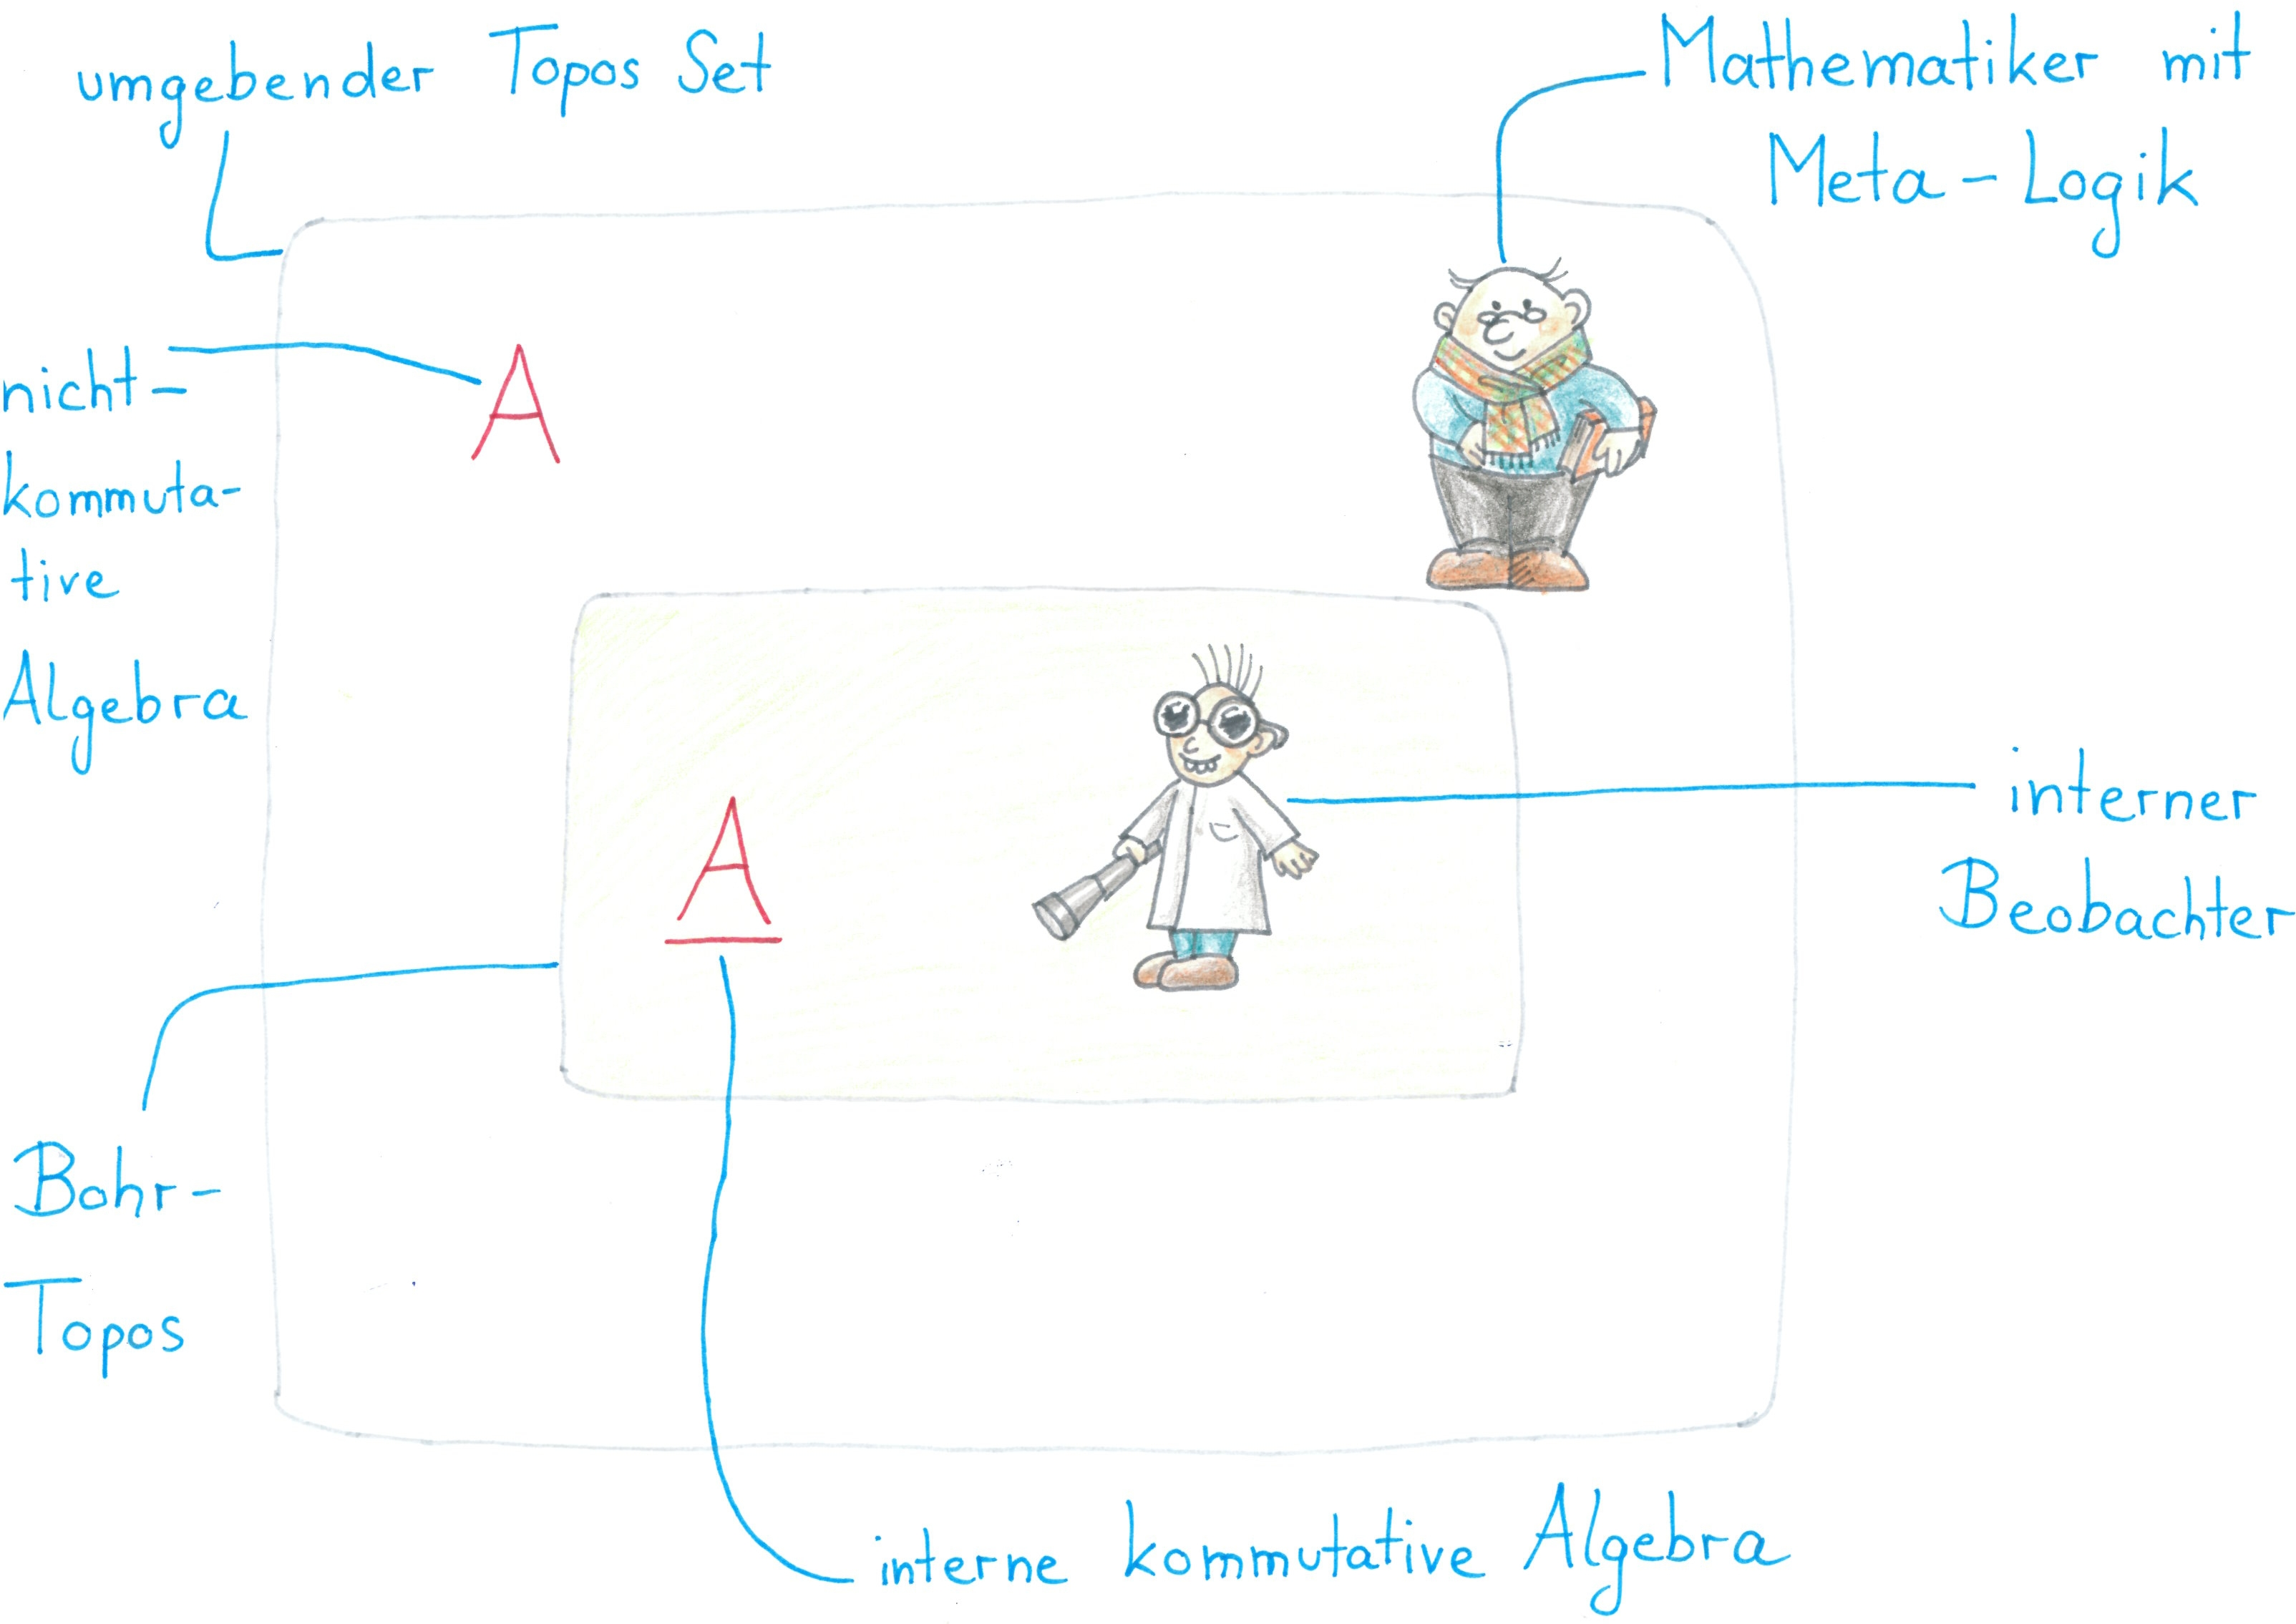
\includegraphics[width=\columnwidth]{bohr-topos}
  \end{block}
  \bigskip

  \begin{block}{Basic example}
    Let~$0 \to \F' \to \F \to \F'' \to 0$ be a short exact sequence of sheaves
    of~$\O_X$-modules. Assume that~$\F'$ and~$\F''$ are of finite type. Then it is
    well-known that~$\F$ is of finite type as well.\medskip

    A sheaf is of finite type if and only if, internally, it is a
    finitely generated module. Therefore the proposition follows \emph{at once}
    by interpreting the analogous statement of intuitionistic linear algebra
    in the little Zariski topos:
    Let~$0 \to M' \to M \to M'' \to 0$ be a short exact sequence of modules.
    If~$M'$ and~$M''$ are finitely generated, so is~$M$.\medskip

    We can thus recognize notions and statements of scheme theory as notions and
    statements of non-sheafy linear algebra.
    \emph{Caveat:} Proofs by contradiction can not be interpreted with the
    internal language.
  \end{block}
\end{column}

\begin{column}{0.3\textwidth}
  \begin{block}{Locally free sheaves}
    Let~$X$ be a reduced scheme. The structure sheaf~$\O_X$ looks like a \emph{field} from the
    internal point of view. This is notable; recall that neither the rings of
    local sections nor the stalks are in general fields.\medskip

    Let~$\F$ be a finite type sheaf of~$\O_X$-modules. 
    Then it is well-known that~$\F$ is locally free on a dense open subset
    of~$X$. (Ravi Vakil, important hard exercise.) \medskip

    This follows \emph{at once} from the following easy proposition of intuitionistic
    linear algebra: Let~$M$ be a finitely generated vector space. Then~$M$ is
    \emph{not not} finite free.
  \end{block}
  \bigskip

  \begin{block}{Rational functions}
    The sheaf~$\K_X$ of rational functions can internally simply be defined as
    the total quotient ring of~$\O_X$.
  \end{block}
  \bigskip

  \begin{block}{Spreading of properties}
    The following metatheorem covers a wide range of cases:
    Let~$\varphi$ be a property which can be formulated without
    using~``$\Rightarrow$'',~``$\neg$'', and~``$\forall$''. Then~$\varphi$
    holds at a point if and only if it holds on some open neighbourhood of the
    point.\medskip

    For instance, a sheaf of modules~$\F$ is zero if and only if, from the
    internal perspective, ``$\forall x \in \F{:}\ x = 0$''. Because of
    the~``$\forall$'', a stalk may be zero without the sheaf being zero on a
    neighbourhood.\medskip

    But if~$\F$ is of finite type, the condition can be reformulated using
    generators as ``$x_1 = 0 \wedge \cdots \wedge x_n = 0$''. The meta-theorem
    is applicable to this statement and thus a stalk is zero if and only if~$\F$
    is zero on a neighbourhood.
  \end{block}

  \vspace{1cm}
  \begin{alertblock}{Dictionary of external vs. internal notions}
    Expository notes are available at \url{http://tiny.cc/topos} (work in
    progress).
  \end{alertblock}
  \tiny\rmfamily\justifying
  Tensor product of sheaves $=$ internal ordinary tensor product,
  internal Cartier divisors,
  quasicoherent sheaves $=$ internal ordinary modules satisfying an interesting
  condition,
  more metatheorems about spreading of properties,
  pullback along immersions $=$ internal sheafification,
  relative spectrum $=$ internal spectrum,
  scheme dimension $=$ Krull dimension of~$\O_X$,
  dense $=$ not not,
  further modal operators,
  other toposes,
  group schemes $=$ groups,
  \ldots
\end{column}

\end{columns}\end{frame}

\end{document}

* own contributions
* "at once"
